\documentclass[13pt]{article}
\usepackage[a4paper, tmargin=1.5cm, lmargin=1.5cm, rmargin=1.5cm, bmargin=1.5cm]{geometry}
\usepackage{hyperref}
%\usepackage{multicol}
\hypersetup{
    colorlinks=true,
    linkcolor=black,
    filecolor=magenta,      
    urlcolor=blue,
    citecolor=black,
}
%\usepackage[numbers,sort&compress]{natbib} % for a numerical citation list
\usepackage{graphicx}
\usepackage{caption}
\usepackage{subcaption} % trong preamble
\usepackage{indentfirst}
\usepackage[utf8]{inputenc}
\usepackage{textcomp}
\usepackage[T1]{fontenc}
\usepackage{CJKutf8}
\usepackage{booktabs}
\usepackage{array}
\usepackage{xcolor}
\usepackage{colortbl}
\usepackage{lmodern}
\usepackage{float}
\usepackage{booktabs}
\usepackage{tikz}
\usepackage{algorithm}
\usepackage{algpseudocode}
\usepackage{amsmath,amssymb} 

\usetikzlibrary{positioning, arrows.meta, calc}

\usepackage{fancyhdr}
\pagestyle{fancy}
\fancyhf{}

\fancyfoot[L]{\footnotesize Bubble Extraction and Dialog Translation for Japanese Manga}
\fancyfoot[R]{\thepage}

\renewcommand{\footrulewidth}{0pt}
\renewcommand{\headrulewidth}{0pt}


%%%%%%%%%%%%%%%%%%%%%%%%%%%%%%%%%%%%%%%%%%%%%%%%%%
%%%%%%%%%%%%%%%%%%%%%%%%%%%%%%%%%%%%%%%%%%%%%%%%%%
%%%%%%%%%%%%%%%%%%%%%%%%%%%%%%%%%%%%%%%%%%%%%%%%%%
%%%%%%%%%%%%%%%%%%%%%%%%%%%%%%%%%%%%%%%%%%%%%%%%%%
%%%%%%%%%%%%%%%%%%%%%%%%%%%%%%%%%%%%%%%%%%%%%%%%%%
%%%%%%%%%%%%%%%%%%%%%%%%%%%%%%%%%%%%%%%%%%%%%%%%%%
\begin{document}
\begin{CJK*}{UTF8}{gbsn}
\pagenumbering{arabic}

\begin{titlepage}
    \thispagestyle{empty}
    \centering
    \vspace{5cm}
    {\Large \textbf{UNIVERSITY OF SCIENCE AND TECHNOLOGY OF HANOI}}\\[0.5cm]
    {\large DEPARTMENT OF INFORMATION AND COMMUNICATION TECHNOLOGY}\\[2cm]

    \includegraphics[width=0.3\linewidth]{img/usth.jpg}
    \\[2cm]

    {\Huge \textbf{Group Project Report}}\\[1cm]
    {\Huge \textbf{Bubble Extraction and Dialog\\[0.5cm] Translation for Japanese Manga}}\\[2cm]

    {\fontsize{16pt}{22pt}\selectfont
    \raggedright
    \begin{tabular}{@{} l l l @{}}
        \textbf{Supervisor} & Assoc. Prof. Tran Giang Son & \\[0.3cm]
        \textbf{Group}      & 49 & \\[0.3cm]
        \textbf{Students}  & Nguyen Lam Tung       & 23BI14446\\
                           & Nguyen Vu Hong Ngoc   & 23BI14345\\
                           & Hoang Khanh Dong      & 22BA13072\\
                           & Le Chi Thanh Lam      & 23BI14248\\
                           & Pham Quang Vinh       & 23BI14455\\
                           & Pham Quang Minh       & 23BI14296\\
    \end{tabular}
    }

\end{titlepage}

\newpage 
\addtocontents{toc}{\protect\setcounter{tocdepth}{-1}}
\section*{List of Abbreviations}
\addtocontents{toc}{\protect\setcounter{tocdepth}{3}}
\begin{table}[H]
    \centering
    \large 
    \begin{tabular}{ll}
        AP & Average Precision \\
        \\
        BERT & Bidirectional Encoder Representations from Transformers \\
        \\
        BLEU & Bilingual Evaluation Understudy \\
        \\
        CER & Character Error Rate \\
        \\
        CNN & Convolutional Neural Network \\
        \\
        COCO & Common Objects in Context \\
        \\
        COMET & Crosslingual Optimized Metric for Evaluation of Translation \\
        \\
        DeBERTa & Decoding-enhanced BERT with Disentangled Attention \\
        \\
        DeiT & Data-efficient Image Transformer \\
        \\
        ELAN & Efficient Layer Aggregation Networks\\
        \\
        FN & False Negatives \\
        \\
        FP & False Positives \\
        \\
        FPN & Feature Pyramid Network \\
        \\
        IoU & Intersection over Union \\
        \\
        JSON & JavaScript Object Notation \\
        \\
        mAP & mean Average Precision \\
        \\
        MSA & Multi-Head Self-Attention \\
        \\
        MT & Machine Translation \\
        \\
        NLP & Natural Language Processing \\
        \\
        OCR & Optical Character Recognition \\
        \\
        PAN & Path Aggregation Network \\
        \\
        RoBERTa & Robustly Optimized BERT Pretraining Approach \\
        \\
        TP & True Positives \\
        \\
        UC & Use Case\\
        \\
        ViT & Vision Transformer \\
    \end{tabular}
\end{table}

\newpage
\thispagestyle{empty}
\tableofcontents
\clearpage


\newpage
\addtocontents{toc}{\protect\setcounter{tocdepth}{-1}}
\centering 
\section*{Abstract}
\addtocontents{toc}{\protect\setcounter{tocdepth}{3}}
Manga translation is a multimodal task that requires both visual understanding and natural language processing.
To support manual manga translation, we present an end-to-end pipeline that assists professional translators by dividing the
process into four main stages: speech bubble segmentation, optical character recognition (OCR), machine translation, and typesetting.

\raggedright
\setlength{\parindent}{1.5em}
\section{Introduction}
Among recent forms of entertainment, digital comics have become increasingly important, especially for young audiences, due to their distinctive hand-drawn art styles and engaging storylines. Comics not only provide entertainment but also foster imagination, creativity, and visual literacy in readers. Their narratives are conveyed primarily through illustrations, making complex ideas and emotions more accessible to younger minds. The diversity of comic content is expanding as creators can easily publish online and reach a wide audience. Manga, a style of comic originating in Japan, has gained significant global popularity—not only for its unique artistic style but also for its rich storytelling and cultural insights.
To make manga accessible to global audiences, translation plays a vital role.\\

However, the process is highly labor-intensive because translators not only interpret the text, but also edit comic pages using graphic tools, remove original dialogues, and replace them with translated content. 
While translation itself is already a demanding task, the additional manual work significantly increases both time and effort, leading to exhaustion, low efficiency, and quality reduction which may impact readers' experience. 
The manual translation workflow typically consists of several stages, as illustrated in Figure \ref{fig:manual_workflow}.
First, translators read the manga to identify key terms and establish a style guide. They then produce translation drafts while continuously updating the glossary.
The final stage is typesetting, which is usually handled by letterers in large translation teams, or by the translators themselves in smaller teams. Images are edited to replace the original text with the translated text.
This repetitive procedure can be exhausting for translators, as manga series are typically released over multiple volumes.\\

With the advancement of technology, comic translation applications were born to support translators and improve workflow efficiency. They can reduce manual workload by automating tasks so that translators can focus on delivering high-quality translations. We propose an end-to-end application supporting professional translators by extracting speech bubbles and text automatically, along with assisted translation features. This work aims to bridge computer vision and natural language processing to perform automatic manga translation.\\

Applying deep learning models and computer vision techniques to manga translation has become a popular topic in academic research. However, practical applications for manga translation are limited and still present several drawbacks for professional translators. Manga Translator \cite{manga_translator}, Comic Translate \cite{comic_translate}, and Mantra Engine \cite{mantra_engine} are representative applications developed for manga translation, corresponding respectively to web, desktop, and mobile platforms.\\

All of these applications offer fast processing with real-time or near–real-time performance, making them suitable for personal use or beginners. Some systems also allow users to select different translation models or support multiple languages, font styles, and image formats. Nevertheless, they share a critical limitation: none of them provide an editing function for the translated text.\\

In addition, Comic Translate \cite{comic_translate} requires users to obtain and configure their own API keys, which can be challenging for non-technical users. The mobile platform, Mantra Engine \cite{mantra_engine}, produces visually unrefined text overlays that often exceed the boundaries of speech bubbles, negatively affecting readability and aesthetic quality.\\

Therefore, our motivation is to develop a platform specifically designed for professional manga translators that provides editing functionality at each stage of the manga translation pipeline. Rather than fully replacing human translators, the application aims to support and enhance manual translation workflows by integrating existing deep learning models and computer vision techniques.

\begin{figure}[H]
    \centering
    \includegraphics[width=1\textwidth]{img/Data-Page-3.pdf}
    \caption{Manual manga translation workflow}
    \label{fig:manual_workflow}

\end{figure}

\section{Related Works}
%early approaches of each stage
Manga translation is not a new research topic since there are many publications working on automatic manga translation.
In 2022, Saikumar et al. \cite{saikumar2022automatic} presented an automated system for translating manga and integrating a multi-stage process into a functional framework.
Authors mentioned a common issue with Japanese while performing translation: Japanese lacks spaces between words and its word ordering in manga (from left to right vertically) are challenging to conventional OCR.
Another paper by Hinami et al. \cite{hinami2021towards} raised another difficulty in context understanding since a character can be divided up into multiple bubbles (narrations) and the order of speech bubbles.




\subsection{Speech Bubble Segmentation}
In 2017,  Rigaud et al. \cite{rigaud2017textindependent} proposed an adaptive thresholding method to binarize grayscale images and extract connected components, identifying speech balloons based on their content topology and alignment. In 2019, Dubray and Laubrock \cite{dubray2019deepcnn} employed a deep convolutional network with a U-Net architecture and a pre-trained VGG-16 encoder to segment speech balloons in comics. Later, Melista et al. (2021) \cite{melistas2021deep} combined Faster R-CNN for balloon bounding box detection with U-Net for pixel-level segmentation of speech balloons.

\subsection{Optical Character Recognition (OCR)}
In text detection and recognition, Hirata et al. \cite{hirata2016comics} employed an image operator learning method generating binary segmentation in pixel level. 
Machine learning algorithms were applied to learn image operators from training images with ground truths, where windows are considered as features.
The choice for window value is important in this task, which can lead to large generalization error. Therefore, two-level operators were born to solve the problem by using moderate size windows for training and combining resulting images.
Later in 2018, Chu et al. \cite{chu2018text} proposed two approaches based on deep networks for text detection.
The first approach utilized multiple CNNs for feature extraction, joined them and fed to a combination of a classification and a regression network.
The other approach took region proposal, extracted features and classification/regression in a single deep network.
While previous studies primarily focus on developing specific text detection or segmentation methods, Soykan et al. \cite{soykan2024comics} provide a comprehensive benchmark and evaluation framework that offers a unified perspective on comics OCR and facilitates systematic comparison across different approaches.

\subsection{Machine Translation}
Manga translation is an increasingly popular topic in applied research; however, there is a lack of academic studies focusing specifically on Japanese-to-English manga translation.
Early in 1986, Nagao et al. \cite{nagao1986mt} described the outline of Japanese to English machine translation system. 
In 2021, Zhou et al. (2021) \cite{zhou2021niutrans} introduced NiuTrans, built on variants of Transformer, Transformer-DLCL (Dynamic Linear Combination of Layers), ODE (Ordinary Differential Equation)-Transformer and vice versa.
Besides, back-translation, knowledge-distillation, post-ensemble and iteractive fine-tuning techniques were applied to improve model performance.
Later in 2024, Kinugawa et al. \cite{Kinugawa2024WMTNonRepetitive} reported the findings of the WMT 2024 shared task on non-repetitive translation, which is particularly relevant to dialogue translation scenarios where avoiding repetitive expressions is crucial.
In the same year, Kaino et al. \cite{kaino2024utilizing} proposed two new approaches to capture contextual information in machine translation for manga: scene-based translation and machine translation incorporating bibliographic attributes: series, author, publisher, magazine and genre.
In manga translation pipelines, translation is typically followed by the typesetting phase, which encompasses both the reinsertion of translated text into speech balloons and the removal of original text to prepare clean background regions. 
Within this context, text removal is a crucial supporting step for typesetting. 
In 2020, Ko et al. \cite{ko2020sickzil} proposed an automated framework for text removal in comics that integrates deep learning with image processing techniques. 
The framework consists of two main stages: pixel-level text segmentation followed by text erasure using inpainting to restore the surrounding visual content.
 
\subsection{Typesetting}
\input{sections/subsections/typesetting-lr}

\section{Methodology}
\subsection{Overall Pipeline}
\begin{figure}[H]
    \centering
    \begin{tikzpicture}[
        % 1. Global Styles
        node distance = 1.5cm and 2cm, % Vertical and Horizontal spacing
        >=Stealth,                       % Nice arrow tip style
        line width=1pt,                  % Thickness of arrows
        % Style for the image nodes
        picnode/.style={
            draw=black,       % Border color (optional, remove if not needed)
            inner sep=0pt,    % No padding between image and border
            outer sep=2pt,    % Space for arrows to touch
        }
    ]

    % -----------------------------------------------------------
    % 2. Define Helper Command for Images
    % Change width/height here to control size
    % -----------------------------------------------------------
    \newcommand{\img}[1]{%
        \includegraphics[width=3cm, height=2cm, keepaspectratio]{#1}%
    }
    
    % --- LEFT COLUMN ---
    \node[picnode] (img1) {\includegraphics[width=8cm]{img/1.png}};
    \node[picnode, below=of img1] (img2) {\includegraphics[width=8cm]{img/2.png}};
    \node[picnode, below=of img2] (img3) {\includegraphics[width=8cm]{img/3.png}};

    % --- RIGHT COLUMN ---
    % Place Image 5 to the right of Image 1
    \node[picnode, right=of img1] (img5) {\includegraphics[width=8cm]{img/5.png}};
    
    % Place Image 4 to the right of Image 3
    \node[picnode, right=of img3] (img4) {\includegraphics[width=8cm]{img/4.png}};

    % Place Image 6 
    \node[picnode, below=of img5] (img6) {\includegraphics[width=8cm]{img/6.png}};

    % -----------------------------------------------------------
    % 3. Draw Arrows
    % -----------------------------------------------------------
    
    % Left Vertical Flow
    \draw[->] (img1) -- node[right, font=\small] {1. Instance Segment} (img2);
    \draw[->] (img2) -- node[right, font=\small] {3. Convex Defect}(img3);

    % Horizontal Connections
    \draw[->] (img2) -- node[right, font=\small] {2. Overlay mask} (img5);
    \draw[->] (img3) -- node[above, font=\small] {4. OCR} (img4);

    % Right Vertical Flow (Sandwich)
    \draw[->] (img5) -- node[right, font=\small] {6. Fill Text}(img6); % Down
    \draw[->] (img4) -- node[right, font=\small] {5. Translation}(img6); % Up

    \end{tikzpicture}
    \caption{Pipeline Workflow}
\end{figure}

\subsection{Dataset}
\label{data}
Manga109 is a dataset compiled by Aizawa Yamasaki Matsui Laboratory, Department of Information and Communication Engineering, the Graduate School of Information Science and Technology, the University of Tokyo \cite{multimedia_aizawa_2020, mtap_matsui_2017}. This dataset consists of 109 manga volumes with their dialog and segmentation annotations, intended for use in academic research.

The dataset contains 10,607 images, of which 9,916 include speech bubbles, with a total of 130,176 bubbles. Segmentation annotations are stored in in COCO-format JSON files. Bubble masks and bounding boxes are stored in Run-Length Encoding (RLE) and [x,y,width,height] formats, correspondingly.
Since RLE is not suitable for model training, evaluating or result visualisation, it must be converted into polygon representations.
In this work, only images containing annotated speech bubbles are used for model training and evaluation. The maximum number of speech bubbles in a single image is 44, and on average, each image contains approximately 13 bubbles, indicating a relatively high bubble density. The bubble distribution following COCO standard is illustrated in Figure \ref{fig:bubble_distribution}.

\begin{figure}[H]
    \centering
    \includegraphics[width=0.7\textwidth]{img/bubble-distribution.png}
    \caption{Speech bubble distribution in Manga109 dataset following COCO standard.}
    \label{fig:bubble_distribution}
\end{figure}

Figure \ref{fig:bubble_distribution} illustrates that speech bubbles considered as large objects make up  46.8\% in total. Medium and small bubbles account for 36.4\% and 16.8\%, respectively. This distribution indicates a significant presence of large speech bubbles in the dataset, which may influence the performance of detection models, as larger objects are generally easier to detect than smaller ones.

\subsection{Bubble Segmentation}
\subsubsection{Pipeline}
The bubble segmentation pipeline processes raw manga pages through three sequential stages to extract individual speech bubble regions suitable for OCR processing.

\begin{figure}[H]
    \centering
    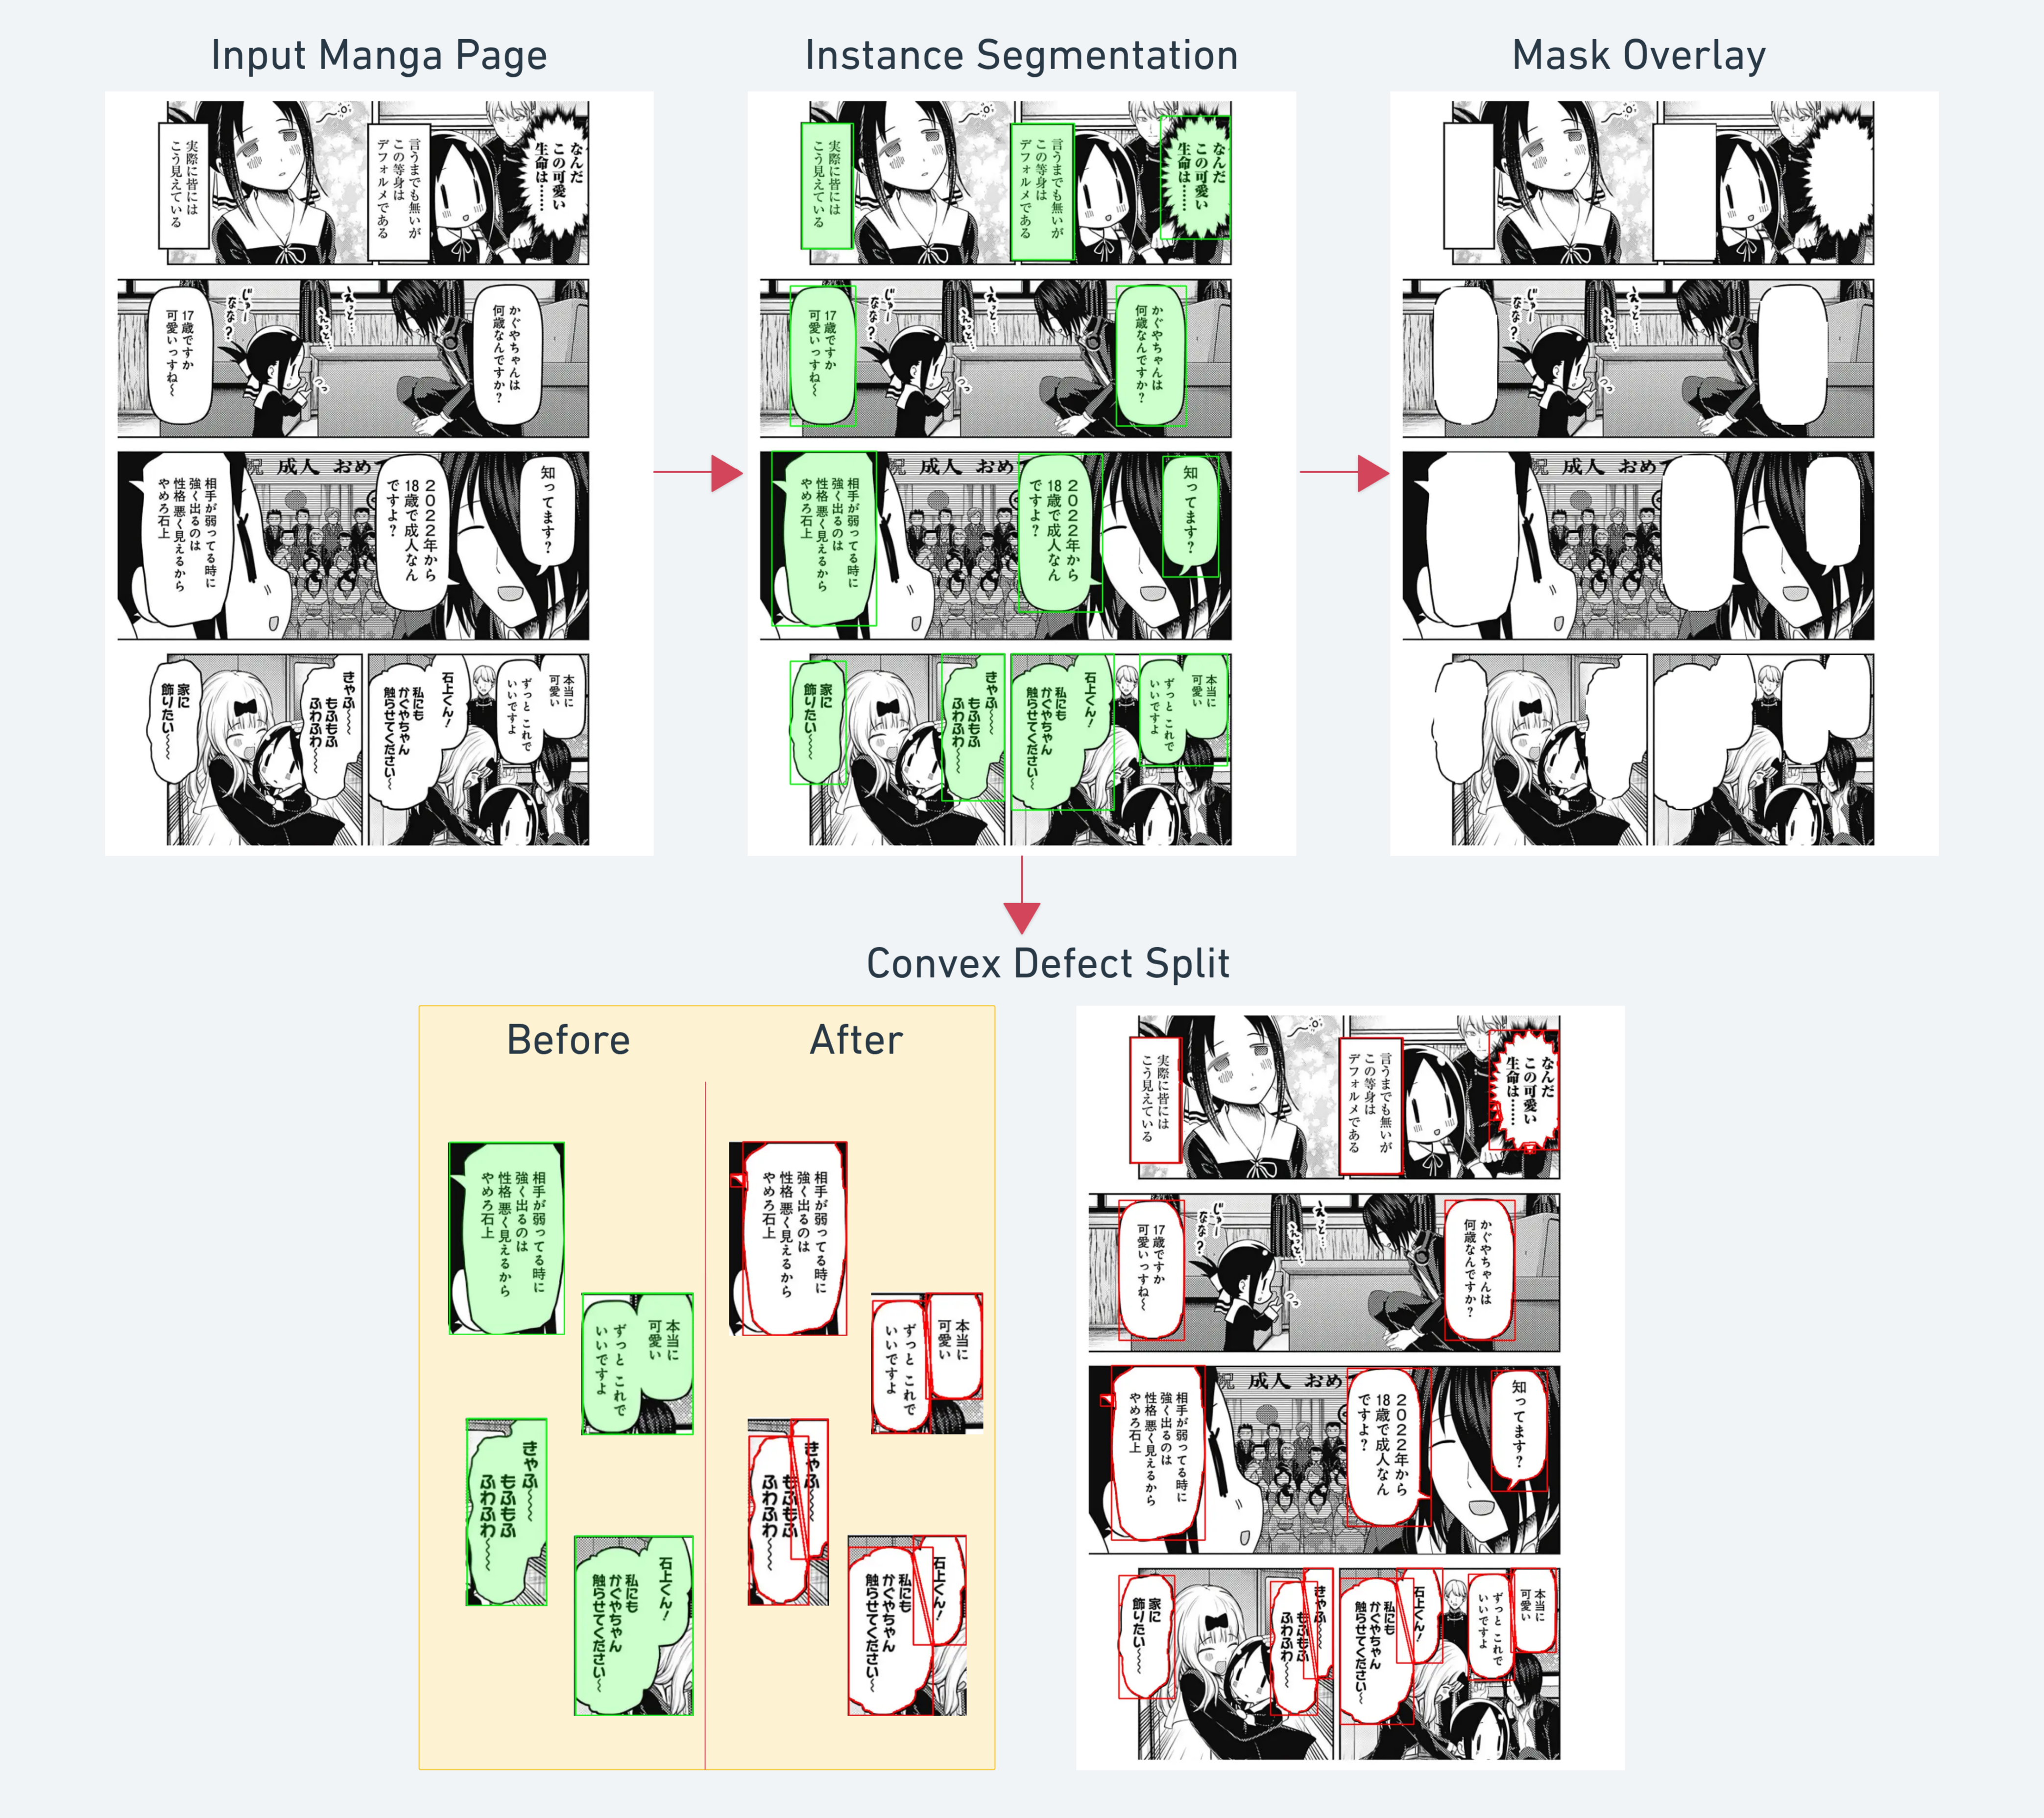
\includegraphics[width=0.9\textwidth]{img/segmentation_pipeline.png}
    \caption{Bubble Segmentation Pipeline}
    \label{fig:bubble-seg-pipeline}
\end{figure}

\subsubsection{Data Preparation}
In this work, Manga109s, a subset of the Manga109 dataset \cite{multimedia_aizawa_2020, mtap_matsui_2017} containing 87 manga volumes, was utilised for model training. In total, the training data consisted of 8649 images with 97896 annotated speech bubbles. The remaining 22 manga titles were used for evaluating, including 1958 images with 29848 annotations.

As mentioned in Section \ref{data}, segmentation annotations follow RLE format, which preserves data integrity and avoids lossy compression. However, this format is not suitable for model  training, evaluating or result visualisation and therefore must be converted into polygon representations.

Each JSON annotation file contains six category identifiers, including our target annotation with category ID equal to 5. To reduce data retrieval time, related information including speech balloon annotations and associated metadata were filtered and stored in a dictionary, where each manga title corresponds to one sub-dictionary.

The dataset was then split and grouped at the manga volume level for training and testing. Images were copied to the corresponding directories and annotations were written to text files for each image. The dataset structure was specified in a YAML configuration file for model training and validation.

Finally, original speech bubble bounding boxes were defined in the [x, y, width, height] format whereas YOLO models expect bounding boxes in the [$x_c$, $y_c$, width, height] format. Therefore, bounding boxes were normalised for storage in text files. During evaluation, YOLO internally converted them into an appropriate representation required for metric computation.




\subsubsection{YOLO Segmentation architecture}
In this study, we employ the YOLO architecture adapted for instance segmentation tasks. Specifically, we investigate two versions: YOLOv8 \cite{10533619} and YOLOv11 \cite{yolo11_ultralytics}.  While both models share a fundamental Anchor-Free, One-Stage detection paradigm, YOLO11 introduces significant architectural refinements to improve feature extraction and processing speed.
The segmentation architecture consists of three primary components: the Backbone, Neck, and Head.

\begin{enumerate}
    \item \textbf{Backbone:} The Backbone is responsible for extracting feature maps from the input manga pages.
YOLOv8 utilises the CSPDarknet structure enhanced with C2f (Cross Stage Partial bottleneck with 2 convolutions) modules. The C2f module improves information flow by merging the concepts of C3 modules \cite{9150780} and ELAN (Efficient Layer Aggregation Networks) \cite{wang2022designingnetwork}.

YOLOv11 replaces the C2f module with the C3k2 block (C3k with a customable kernel size). Furthermore and integrates the C2PSA (Convolutional Block with Parallel Spatial Attention) module at the end of the backbone \cite{yolo11_ultralytics}. This attention mechanism allows the model to focus more effectively on spatial features such as the contours of a bubble against complex manga backgrounds before passing data to the Neck. 
The architectures of the C2PSA module, the attention block in YOLOv11, the C2f module, and the C3k2 module are illustrated in Figures \ref{fig:c2psa_psablock} \cite{hidayatullah2025yolov8_yolo11_review} and \ref{fig:c2f_c3k2}  \cite{hidayatullah2025yolov8_yolo11_review}.

\begin{figure}[H]
    \centering
    \begin{subfigure}{0.48\textwidth}
        \centering
        \includegraphics[width=0.9\linewidth]{img/C2PSA.png}
        \caption{C2PSA module}
    \end{subfigure}
    \hspace{-1.5em}
    \begin{subfigure}{0.48\textwidth}
        \centering
        \includegraphics[width=0.7\linewidth]{img/PSABlock.png}
        \caption{Attention block (YOLOv11)}
    \end{subfigure}
    \caption{Architecture of PSA-based modules: (a) C2PSA module; (b) Attention block used in YOLOv11 \cite{hidayatullah2025yolov8_yolo11_review}}
    \label{fig:c2psa_psablock}
\end{figure}


\begin{figure}[H]
    \centering
    \begin{subfigure}{0.48\textwidth}
        \centering
        \includegraphics[width=0.9\linewidth]{img/C2f.png}
        \caption{C2f module}
    \end{subfigure}
    \hspace{-1.5em}
    \begin{subfigure}{0.48\textwidth}
        \centering
        \includegraphics[width=0.7\linewidth]{img/C3k2.png}
        \caption{C3k2 module (YOLOv11)}
    \end{subfigure}
    \caption{Comparison of backbone modules: (a) C2f module; (b) C3k2 module adopted in YOLOv11 \cite{hidayatullah2025yolov8_yolo11_review}}
    \label{fig:c2f_c3k2}
\end{figure}

    \item \textbf{Neck (Feature Fusion):} Both versions employ a PANet (Path Aggregation Network) \cite{8579011} structure combined with an FPN (Feature Pyramid Network) \cite{8099589}. This component aggregates features from different backbone stages. Since manga bubbles can range from tiny whispers to page-dominating shouts, this multi-scale fusion is critical for detecting instances of all sizes effectively.
    \item \textbf{Segmentation Head for Mask Generation:} Unlike standard object detection, the output of segmentation head is pixel-wise mask, followed by Decoupled Head architecture \cite{ge2021yoloxexceedingyoloseries}, which separates the classification and regression tasks.
    
    Following the YOLACT (You Only Look At Coefficients) principle \cite{9010373}, the mask generation pipeline begins with Protonet, a dedicated branch that learns a fixed set of k prototype masks—generic bases that are shared across every image and never conditioned on any particular object. Concurrently, the detection head predicts, for each anchor, k scalar mask coefficients that encode the instance-specific contribution of every prototype. These coefficients are multiplied with their corresponding prototypes, the weighted maps are summed, a sigmoid activation converts the logits to per-pixel probabilities, and the resulting mask is finally cropped to the predicted bounding box to produce the assembled instance mask.
    The architecture of YOLACT is illustrated in Figure \ref{fig:yolo-segmentation-head}.

    \begin{figure}[H]
        \centering
        \includegraphics[width=0.7\linewidth]{img/YOLACT.png}
        \caption{YOLACT architecture}
        \label{fig:yolo-segmentation-head}
    \end{figure}

\end{enumerate}


\subsubsection{Model Training}
Four YOLO models—YOLOv8s, YOLOv8n, YOLOv11s, and YOLOv11n—were trained using the same hyper-parameters, as shown in Table \ref{tab:yolo-hyperparams}. Apart from the defined hyper-parameters, all other training settings remained unchanged. In each epoch, images were processed in batches in parallel. Images were resized to the selected input resolution, as specified in Table \ref{tab:yolo-hyperparams} and then forwarded through the layers of the YOLO models. After each epoch, the validation loss was computed, and the model achieving a lower validation loss than the current best was saved as the best-performing model. Model parameters were updated via back propagation and used in the next epoch.

\begin{table}[htbp]
\centering
\label{tab:yolo-hyperparams}
\begin{tabular}{lc}
\toprule
Hyper-parameter & Value \\
\midrule
Epochs     & 10 \\
Image size & $1280 \times 1280$ \\
Batch size & 4 \\
\bottomrule
\end{tabular}
\caption{Training hyper-parameters for YOLO models}
\end{table}



\subsubsection{Post-processing for speech bubbles}
Although YOLO gives a a pixel-precise mask for every panel, it still returns \textbf{one} mask when two, three or more balloons touch or overlap. Feeding such a merged region to an OCR engine makes the text layout denser and usually causes a noticeable drop in recognition accuracy.

To address this, we introduce a post-processing step that leverages convexity defects to detect and split merged speech bubbles. The key observation is that when two bubbles are connected, the resulting contour often exhibits at least two deep concave regions — known as convexity defects. These defects serve as reliable cues for where a cut should be made.

Our algorithm proceeds as follows: for each mask returned by YOLO we extract the largest external contour, compute its convex hull and identify convexity defects—points where the contour deviates markedly from its convex envelope—retaining only those that are both deep and angularly valid to suppress noise, then merge nearby defects to avoid over-segmentation; subsequently we draw a straight line between the closest pair of defects if at least two valid ones remain, whereas if only a single valid defect exists we skip the cut entirely since one defect alone does not furnish sufficient geometric evidence for a reliable split, and the entire process is applied recursively to each resulting sub-mask up to a predefined depth to handle more complex multi-bubble clusters.

\begin{algorithm}[H]
\caption{Split Merged Speech Bubbles Using Convexity Defects (Conservative)}
\begin{algorithmic}[1]
\Procedure{SplitBubbles}{$mask$, $depth$}
    \If{$depth \geq \text{MAX\_DEPTH}$}
        \State \Return $[mask]$
    \EndIf
    \State $contour \gets \text{LargestContour}(mask)$
    \If{$\text{Area}(contour) < 500$}
        \State \Return $[mask]$
    \EndIf
    \State $hull \gets \text{ConvexHull}(contour)$
    \State $defects \gets \text{ConvexityDefects}(contour, hull)$
    \State $candidates \gets \emptyset$
    \For{$defect \in defects$}
        \State $(s, e, f, d) \gets defect$
        \State $depth\_val \gets d / 256.0$
        \If{$depth\_val > \text{MIN\_DEFECT\_DEPTH}$}
            \State $angle \gets \text{AngleBetween}(s, f, e)$
            \If{$angle < \text{MAX\_ANGLE}$}
                \State $candidates \gets candidates \cup \{f\}$
            \EndIf
        \EndIf
    \EndFor
    \State $candidates \gets \text{ClusterAndFilter}(candidates)$
    \State $cut\_mask \gets mask$
    \If{$|candidates| \geq 2$}
        \State $(p1, p2) \gets \text{ClosestPair}(candidates)$
        \State $\text{DrawLine}(cut\_mask, p1, p2, 0, 3)$
        \State \Return $[mask]$
    \EndIf
    \State $sub\_masks \gets \text{ExtractContours}(cut\_mask)$
    \If{$|sub\_masks| > 1$}
        \State $result \gets \emptyset$
        \For{$sub \in sub\_masks$}
            \State $result \gets result \cup \text{SplitBubbles}(sub, depth + 1)$
        \EndFor
        \State \Return $result$
    \Else
        \State \Return $[mask]$
    \EndIf
\EndProcedure
\end{algorithmic}
\end{algorithm}

Where \textit{s}, \textit{e}, and \textit{f} denote the starting point, ending point, and the furthest point inside the defect, respectively. 
The defect depth \textit{d} is calculated as the distance from point \textit{f} to the line segment connecting \textit{s} and \textit{e}, encoded as an integer.



\subsection{Optical Character Recognition (OCR)}
To translate the visual content of speech bubbles into machine-readable text, we integrate the \textbf{MangaOCR} framework. While general-purpose OCR engines (e.g., Tesseract) struggle with the non-linear layout and unique typography of Japanese manga, MangaOCR is specifically architected to handle vertical text, \textbf{furigana} (pronunciation guides), and mixed writing systems.

\subsubsection{Model architecture}
We utilize the official pre-trained weights of the \texttt{manga-ocr-base} model. Training a robust manga OCR model from scratch requires generating millions of synthetic image-text pairs and significant computational resources to converge. By leveraging the pre-trained model, which has already learned high-level feature representations from extensive synthetic datasets (based on CC-100 corpus and Manga109), we achieve state-of-the-art performance without the overhead of training.
The architecture of the Manga-OCR model is illustrated in Figure \ref{fig:manga-ocr-architecture}.

\begin{figure}[!ht]
    \centering
    \includegraphics[width=0.9\textwidth]{img/manga-ocr-pipeline.pdf}
    \caption{Manga-OCR Model Architecture}
    \label{fig:manga-ocr-architecture}
\end{figure}


The model follows a \textbf{Vision Encoder-Decoder} architecture with approximately 115 million parameters:

\begin{enumerate}
    \item \textbf{Vision Encoder (ViT):} The backbone is a Data-efficient Image Transformer (DeiT-Tiny) \cite{touvron2021deit} with 12 layers. It processes the input manga bubble image (224$\times$224 pixels) by first splitting it into 196 non-overlapping patches of $16 \times 16$ pixels each. Each patch is converted into a 768-dimensional embedding vector and augmented with positional information to preserve spatial relationships. The patch sequence then passes through 12 Transformer encoder layers, where Multi-Head Self-Attention (MSA) mechanisms capture both local character strokes and global text layout patterns. The output is a set of visual features $H_{\text{enc}}$ that encode the entire image content.
    
    \item \textbf{Text Decoder (BERT):} The decoder is a Japanese character-level BERT model \cite{devlin2018bert} adapted for autoregressive text generation. It generates characters one at a time by processing previously generated text (context tokens) through masked self-attention layers, ensuring each prediction only depends on prior characters. The decoder's key innovation is the \textbf{Cross-Attention} mechanism, which connects visual features $H_{\text{enc}}$ from the encoder to the text generation process in $H_{\text{dec}}$. This mechanism allows the model to focus on relevant parts of the image---such as specific character strokes---when predicting each character. The attention operation is computed as:
    \begin{equation}
        Q = H_{\text{dec}} W_Q, \quad K = H_{\text{enc}} W_K, \quad V = H_{\text{enc}} W_V
    \end{equation}
    \begin{equation}
        \text{Attention}(Q, K, V) = \text{softmax}\left(\frac{QK^T}{\sqrt{d_k}}\right)V
    \end{equation}
    
    After cross-attention integrates visual information with textual context, the final hidden state passes through a linear projection (LM Head) that maps to the vocabulary of 4,718 Japanese characters, followed by softmax to produce probability distributions over the next character.
\end{enumerate}

Where $Q$ (Query) denotes the textual context from decoder states $H_{\text{dec}}$;
$K$ (Key) and $V$ (Value) denote visual features from encoder states $H_{\text{enc}}$;
$W_Q$, $W_K$, and $W_V$ are learnable projection matrices; and
$d_k$ is the key dimensionality used for gradient stabilization.

\subsubsection{Inference algorithm}
The inference pipeline transforms the raw crops from the segmentation module into a coherent dialogue transcript.

We employ a centroid-based algorithm to map text annotations to bubble regions. Let $b$ be a detected bubble mask and $t$ be a text bounding box with center $C(x, y)$. The association function $f(t, b)$ is defined as:
\begin{equation}
    f(t, b) = \begin{cases}
    1 & \text{if } C(x,y) \in \text{Area}(b), \\
    0 & \text{otherwise}
    \end{cases}
\end{equation}

For each sorted crop, we generate text using \textbf{Beam Search} (width $k=4$). We apply a length penalty $alpha=2.0$ to the scoring function to encourage the generation of complete sentences, ensuring that longer dialogue lines are not truncated prematurely.

\subsubsection{Post-processing for OCR results}
The raw output generated by the OCR model often contains artifacts inherent to stochastic decoding, such as irregular whitespace and inconsistent character encodings. To ensure high-quality input for the subsequent translation module, we implemented a deterministic cleaning pipeline utilizing regular expressions and Unicode normalization.

The process applies the following transformations sequentially:
\begin{enumerate}
\item \textbf{Unicode Normalization (NFKC):} Standardizes character widths by converting full-width alphanumeric characters (e.g., \begin{CJK}{UTF8}{min}1 A\end{CJK}) into their canonical half-width counterparts (``1'', ``A'').
\item \textbf{Whitespace Removal:} Eliminates phantom spaces inserted between characters, as Japanese writing does not rely on whitespace for word delimitation.
\item \textbf{Punctuation Standardization:}
Collapses sequences of multiple periods into a single ellipsis (...) and
normalizes tildes (\textasciitilde) to the Japanese wave dash (U+301C) to maintain typographic consistency.
\end{enumerate}

The impact of this pipeline is demonstrated in Table \ref{tab:ocr_cleaning}.

\begin{table}[H]
\centering
\caption{Comparison of Raw OCR outputs against Post-processed text and Ground Truth.}
\label{tab:ocr_cleaning}

\setlength{\tabcolsep}{8pt}
\renewcommand{\arraystretch}{1.3}

\begin{CJK}{UTF8}{min}
\begin{tabular}{>{\raggedright\arraybackslash}p{0.3\textwidth}
                >{\raggedright\arraybackslash}p{0.3\textwidth}
                >{\raggedright\arraybackslash}p{0.3\textwidth}}
\toprule
\rowcolor[HTML]{EFEFEF}
\textbf{Ground Truth} & \textbf{Raw OCR Output} & \textbf{Post-processed Text} \\
\midrule
爆発まで残り 04:30:21 &
爆発まで残り、 D4:30:21 &
爆発まで残り、D4:30:21 \\

なっななな\ldots 何やってんの!? &
なっななな\ldots 何やってんの!? &
なっななな\ldots 何やってんの!? \\

うへ\textasciitilde\textasciitilde!? なんじゃ &
うへ \textasciitilde{} \textasciitilde{} !? なんじゃ &
うへ\textasciitilde\textasciitilde!? なんじゃ \\

ファンクラブ規約No.13 &
ファンクラブ規約 No.13 &
ファンクラブ規約No.13 \\
\bottomrule
\end{tabular}
\end{CJK}
\end{table}


\subsection{Translation}
For translation, we used Neural Machine Translation (NMT) to convert the extracted Japanese text into English text. We utilised the 'elan-mt-ja-en' model series provided by Mitsua, which is built upon the MarianMT framework 
\cite{junczysdowmunt2018marian}.
The underlying architechture of the model family is a standard Transformer encoder-decoder network \cite{vaswani2017attention}.

\subsubsection{Model architecture}
\begin{figure}[H]
    \centering
    \includegraphics[width=0.8\textwidth]{img/marian.png}
    \caption{Marian-MT architecture}
    \label{fig:translation-arch}    
\end{figure}

The MarianMT architecture, illustrated in Figure \ref{fig:translation-arch}, follows the original Transformer design, consisting of an encoder that processes the source Japanese text and a decoder that generates the target English translation autoregressively. The encoder employs multi-head self-attention layers to capture contextual relationships within the input sequence, while the decoder uses both self-attention and cross-attention mechanisms to attend to relevant encoder representations during generation.

The model utilizes SentencePiece tokenization \cite{kudo-richardson-2018-sentencepiece}, a subword segmentation approach that handles the morphologically rich nature of Japanese text by decomposing words into smaller units. This enables the model to handle rare words and out-of-vocabulary tokens effectively while maintaining a manageable vocabulary size.

\subsubsection{Model variants}
We integrate three specific variants of the model to balance translation quality and computational efficiency, as shown in
Table \ref{tab:translation-variants}.

\begin{table}[H]
    \centering
    \begin{tabular}{|c|c|l|}
        \hline
        \textbf{Model Name} & \textbf{Parameters} & \textbf{Description} \\
        \hline
        Mitsua/elan-mt-bt-ja-en & 61M & Back-translation augmented variant with \\
        & & improved handling of colloquial expressions\\
        \hline
        Mitsua/elan-mt-base-ja-en & 61M & Base model trained on parallel corpora \\
        \hline
        Mitsua/elan-mt-tiny-ja-en & 15M & Lightweight variant optimized for inference speed \\
        \hline
    \end{tabular}
    \caption{Variants of the Mitsua/elan-mt model family}
    \label{tab:translation-variants}

\end{table}

The \textbf{bt} (back-translation) variant employs data augmentation through synthetic parallel data generation, where monolingual English text is translated back to Japanese to create additional training pairs

The \textbf{tiny} variant reduces the model depth and hidden dimensions, achieving approximately 4× parameter reduction while maintaining reasonable translation quality. This variant is suitable for resource-constrained environments or applications requiring real-time inference.

\subsection{Typesetting}
% fix

Typesetting is the final step in the manga translation pipeline. It takes the output of the post-processor and uses it to typeset the text in the panel. The typesetter is a simple function that takes a mask and a list of bounding boxes as input and returns a list of typesetted text. The typesetter uses the bounding boxes to determine the layout of the text and the mask to determine the content of the text.

\begin{table}[H]
\centering
\begin{tabular}{|c|l|}
    \hline
    \textbf{Component} & \textbf{Purpose} \\
    \hline
    Whitening & Erasing the original Japanese characters by filling the eroded mask region with white pixels.\\
    \hline 
    Text Rendering & Rendering the text in the bubble mask.\\
    \hline
    Collision Detection & Ensuring that the rendered text does not collide with the bubble boundary.\\
    \hline
    Typesetting & Typesetting the text in the bubble mask.\\
    \hline
\end{tabular}
\caption{Typesetting Module Components}
\end{table}

The typesetting pipeline operates in two sequential phases. In the whitening phase illustrated in Algorithm \ref{alg:render_bubb}, we iterate over each bubble that contains translated text and erase the original Japanese characters by filling the eroded mask region with white pixels. Erosion with a $6 \times 6$ kernel prevents the fill from bleeding into the bubble's border, preserving the visual integrity of the speech balloon outline.

The text rendering phase employs an adaptive font-sizing strategy. Starting from the largest feasible font size (the minimum of the bounding box's height and width), we progressively reduce the size in decrements of 2 until the wrapped text fits entirely within the bubble mask. The SmartWrapText function in Algorithm \ref{alg:smart-wrap} handles word-level wrapping first; if a single word exceeds the available width, it falls back to character-level breaking to ensure no text overflows.

To guarantee that rendered text does not collide with the bubble boundary, we perform pixel-level collision detection described in Algorithm \ref{alg:collision-detect} and \ref{alg:collision-mask}: the text block is temporarily drawn onto a blank canvas, and a bitwise and operation checks whether any text pixels overlap with the inverted bubble mask (i.e., the "wall" region outside the bubble). If collision is detected, we reduce the font size and retry. Should no valid size be found above the minimum threshold of 12 pixels, the algorithm renders the text at the minimum size regardless—ensuring the translation is always visible, albeit potentially clipped.

Finally, the text is drawn centered on the bubble's centroid $(c_x, c_y)$, yielding a natural, balanced appearance consistent with professional manga typesetting conventions.



\begin{algorithm}[H]
\caption{Render Translated Bubbles}
\label{alg:render_bubb}
\begin{algorithmic}[1]
\Function{Render}{$I_{\text{original}}, B$}
    \State $I_{\text{final}} \gets$ copy($I_{\text{original}}$)
    \State $K_{\text{erosion}} \gets$ ones($6 \times 6$)

    \Statex{Phase 1: Whitening (Inpainting) Step}
    \ForAll{$b \in B$}
        \If{$b.\text{translated\_text}$ is empty}
            \State \textbf{continue}
        \EndIf
        \State $M \gets b.\text{original\_mask} \text{ or } b.\text{mask}$
        \State $M_{\text{eroded}} \gets \text{Erode}(M, K_{\text{erosion}})$
        \State $C \gets \text{FindContours}(M_{\text{eroded}})$
        \State \text{FillContours}($I_{\text{final}}, C, \text{white}$)
    \EndFor

    \Statex{Phase 2: Text Rendering Step}
    \State $I_{\text{pil}} \gets \text{ConvertToPIL}(I_{\text{final}})$
    \State $D \gets \text{CreateDrawContext}(I_{\text{pil}})$

    \ForAll{$b \in B$}
        \If{$b.\text{translated\_text}$ is not empty}
            \State \text{FitText}($D, b.\text{translated\_text}, b.\text{mask}$)
        \EndIf
    \EndFor

    \State \Return \text{ConvertToNumpy}($I_{\text{pil}}$)
\EndFunction
\end{algorithmic}
\end{algorithm}

\begin{algorithm}[H]
\caption{Smart Word Wrapping}
\label{alg:smart-wrap}
\begin{algorithmic}[1]
\Function{SmartWrapText}{$D, T, F, W_{\text{max}}$}
    \State $words \gets \text{Split}(T)$
    \State $L \gets []$  \Comment{List of wrapped lines}
    \State $current\_line \gets []$

    \ForAll{$w \in words$}
        \State $test\_line \gets \text{Join}(current\_line + [w], \text{space})$
        \State $width \gets \text{MeasureTextWidth}(D, test\_line, F)$

        \If{$width \leq W_{\text{max}}$}
            \State Append $w$ to $current\_line$
        \Else
            \If{$current\_line \neq []$}
                \State Append Join($current\_line$, space) to $L$
                \State $current\_line \gets [w]$
            \Else
                \Statex{Force character-level breaking}
                \State $temp \gets ""$
                \ForAll{$c \in w$}
                    \If{$\text{MeasureTextWidth}(D, temp+c, F) \leq W_{\text{max}}$}
                        \State $temp \gets temp + c$
                    \Else
                        \State Append $temp$ to $L$
                        \State $temp \gets c$
                    \EndIf
                \EndFor
                \State $current\_line \gets [temp]$
            \EndIf
        \EndIf
    \EndFor

    \If{$current\_line \neq []$}
        \State Append Join($current\_line$, space) to $L$
    \EndIf

    \State \Return $L$
\EndFunction
\end{algorithmic}
\end{algorithm}

\begin{algorithm}[H]
\caption{Fit Text in Mask with Collision Detection}
\label{alg:collision-detect}
\begin{algorithmic}[1]
\Function{FitTextInMask}{$D, T, M$}
    \State $C \gets \text{FindContours}(M)$
    \If{$C = \emptyset$} \State \Return \EndIf

    \State $cnt \gets \text{LargestContourByArea}(C)$
    \State $(x, y, w, h) \gets \text{BoundingRect}(cnt)$
    \State $(c_x, c_y) \gets \text{ComputeCentroid}(cnt)$
    \State $M_{\text{crop}} \gets M[y:y+h, x:x+w]$

    \Statex{Attempt 1: Pixel-Perfect Fit with Binary Search}
    \State $s_{\text{font}} \gets \min(h, w)$
    \State $s_{\min} \gets 12$
    \State $font_{\text{best}} \gets \text{null}$

    \While{$s_{\text{font}} \geq s_{\min}$}
        \State $F \gets \text{LoadFont}(s_{\text{font}})$
        \State $L \gets \text{SmartWrapText}(D, T, F, 0.95 \times w)$
        \State $H_{\text{text}} \gets \sum_{l \in L} \text{TextHeight}(l, F)$

        \If{$H_{\text{text}} > h$}
            \State $s_{\text{font}} \gets s_{\text{font}} - 2$
            \State \textbf{continue}
        \EndIf

        \Statex{Collision Detection via Mask Rendering}
        \State $Canvas \gets \text{CreateCanvas}(w, h, \text{black})$
        \State $y_{\text{curr}} \gets (c_y - y) - H_{\text{text}}/2$

        \ForAll{$l \in L$}
            \State RenderText($Canvas, l, (c_x - x - w_l/2, y_{\text{curr}}), F, \text{white}$)
            \State $y_{\text{curr}} \gets y_{\text{curr}} + \text{TextHeight}(l, F)$
        \EndFor

        \If{not CheckMaskCollision($Canvas, M_{\text{crop}}$)}
            \State $font_{\text{best}} \gets F$
            \State $lines_{\text{best}} \gets L$
            \State $y_{\text{start}} \gets c_y - H_{\text{text}}/2$
            \State \textbf{break}
        \Else
            \State $s_{\text{font}} \gets s_{\text{font}} - 2$
        \EndIf
    \EndWhile

    \Statex{Attempt 2: Fallback - Force Render at Minimum Size}
    \If{$font_{\text{best}} = \text{null}$}
        \State $font_{\text{best}} \gets \text{LoadFont}(s_{\min})$
        \State $lines_{\text{best}} \gets \text{SmartWrapText}(D, T, font_{\text{best}}, w)$
        \State $H_{\text{text}} \gets \sum_{l \in lines_{\text{best}}} \text{TextHeight}(l, font_{\text{best}})$
        \State $y_{\text{start}} \gets c_y - H_{\text{text}}/2$
    \EndIf

    \Statex{Final Rendering}
    \State $y_{\text{curr}} \gets y_{\text{start}}$
    \ForAll{$l \in lines_{\text{best}}$}
        \State $w_l \gets \text{TextWidth}(l, font_{\text{best}})$
        \State DrawText($D, l, (c_x - w_l/2, y_{\text{curr}}), font_{\text{best}}, \text{black}$)
        \State $y_{\text{curr}} \gets y_{\text{curr}} + \text{TextHeight}(l, font_{\text{best}})$
    \EndFor
\EndFunction
\end{algorithmic}
\end{algorithm}

\begin{algorithm}[H]
\caption{Mask Collision Detection}
\label{alg:collision-mask}
\begin{algorithmic}[1]
\Function{CheckMaskCollision}{$M_{\text{text}}, M_{\text{bubble}}$}
    \State $M_{\text{wall}} \gets \text{BitwiseNot}(M_{\text{bubble}})$ \Comment{White = Wall boundary}
    \State $M_{\text{overlap}} \gets \text{BitwiseAnd}(M_{\text{text}}, M_{\text{wall}})$
    \State \Return $\text{CountNonZero}(M_{\text{overlap}}) > 0$
\EndFunction
\end{algorithmic}
\end{algorithm}




\subsection{Evaluation metrics}
\subsubsection{Segmentation}
As the proposed approach addresses an instance segmentation task, all four YOLO models are evaluated using the standard COCO evaluation protocol, reporting Precision, Recall, mAP50, and $mAP@[0.5:0.95]$ for both bounding box detection and mask segmentation. Precision and Recall are defined as:

\begin{equation}
    Precision = \frac{TP}{TP + FP}
\end{equation}
\begin{equation}
    Recall = \frac{TP}{TP + FN}
\end{equation}

Where TP, FP, and FN denote True Positives, False Positives, and False Negatives, respectively. A prediction is considered a true positive if its IoU with the ground-truth instance exceeds a predefined threshold; otherwise, it is counted as a false positive. Ground-truth bubbles that are not matched by any prediction are treated as false negatives.\\

Average Precision (AP) is computed as the area under the precision--recall curve. mAP\@50 denotes the mean AP at an Intersection over Union (IoU) threshold of 0.50, while $mAP@[0.5:0.95]$ averages AP over IoU thresholds from 0.50 to 0.95 with a step size of 0.05.

\subsubsection{Natural Language Processing metrics}
For NLP tasks like OCR and Translation we use Word Error Rate (WER), Character Error Rate (CER) and BLEUScore as the primary metrics for text OCR pipeline, for Jp-En translation pipeline we use BLEUScore and chrF++ metrics.

\begin{enumerate}
    \item  \textbf{Word Error Rate (WER)}

    WER is widely used to evaluate the accuracy of translation and transcription systems. It is derived as the Levenshtein distance from the predicted text and the reference text divided by total number of words in the reference text, the metric is formulated as follow:

    \begin{equation}
        WER = \frac{S + D + I}{N}
    \end{equation}

    Where S (Substitution) is the number of words incorrectly recognized as different words, D (Deletion) is the number of words present in the reference but missing in the prediction, I (Insertion) is the number of extra words present in the prediction but not in the reference.

    \item \textbf{Character Error Rate (CER)}

    CER is derived as the Levenshtein distance from the translated text and the reference text divided by total number of character in the reference text, the metric is formulated as follow:

    \begin{equation}
        CER = \frac{S + D + I}{N}
    \end{equation}

    Where S (Substitution) is the number of character incorrectly recognized as different character, D (Deletion) is the number of characters present in the reference but misssing in the prediction, I (Insertion) is the number of extra characters present in the prediction but not in the reference. For Japanese to English translation, CER is more prefered than WER (Word Error Rate).

    \item \textbf{BLEU Score}
    The Bilingual Evaluation Understudy (BLEU) score is the standard metric for evaluating the quality of machine-translated text against human reference translations. It measures the correspondence between the machine's output and the professional translation based on n-gram overlap.

    \begin{equation}
        BLEU = BP \cdot exp \left( \sum_{n=1}^{N} w_n \log p_n \right)  
    \end{equation}

    Where $p_n$ is the modified n-gram precision, which measures the fraction of n-grams (sequences of $n$ words) in the candidate text that also appear in the reference text. Standard BLEU typically uses 1-gram to 4-gram overlaps ($N=4$). $w_n$ is the weight assigned to each n-gram level, typically set uniformly ($1/N$).
    BP (Brevity Penalty) is a multiplicative factor that penalizes translations that are significantly shorter than the reference. This prevents the model from achieving artificially high precision scores by outputting only a few safe words.

    \item \textbf{Character n-gram F-score (chrF)}

    The Character n-gram F-score (chrF) is an evaluation metric that assesses the quality of machine translation by calculating the F-score of character n-gram overlaps between the hypothesis and the reference. Unlike BLEU, which operates at the word level, chrF works at the character level, making it particularly robust for morphologically rich languages and less sensitive to tokenization errors.

    \begin{equation}
        chrF = \frac{(1 + \beta^2) \cdot chrP \cdot chrR}{\beta^2 \cdot chrP + chrR}
    \end{equation}

    Where "chrP" (Character Precision) refers to the percentage of character n-grams in the system output that are also present in the reference, and "chrR" (Character Recall) refers to the percentage of character n-grams in the reference that are present in the system output. The parameter $\beta$ controls the weight given to recall versus precision; typically, $\beta=2$ is used (often called chrF++) to emphasize recall.
\end{enumerate}

\section{Results and Evaluation}
\subsection{Bubble Segmentation}
Table \ref{tab:yolo-det-per} and Table \ref{tab:yolo-seg-per} illustrate bounding box and instance mask segmentation of four YOLO models: YOLOv8s, YOLOv8n, YOLOv11s, YOLOv11n.
\begin{table}[H]
\centering
\begin{tabular}{lcccc}
\toprule
Model\ /Metrics & YOLOv8n & YOLOv8s & YOLOv11n & YOLOv11s \\
\midrule
Precision & 0.973 & 0.974 & 0.974 & \textbf{0.977} \\
Recall & 0.978 & \textbf{0.982} & 0.977 & 0.978\\
mAP50 & 0.992 & \textbf{0.993} & 0.992 & \textbf{0.993}\\
mAP50-95 & 0.97 & 0.974 & \textbf{0.979} & 0.975\\
\bottomrule
\end{tabular}
\caption{Bubble bounding box detection performance of YOLO models}
\label{tab:yolo-det-per}
\end{table}

\vspace{0.5cm}

\begin{table}[H]
\centering
\begin{tabular}{lcccc}
\toprule
Model\ /Metrics & YOLOv8n & YOLOv8s & YOLOv11n & YOLOv11s \\
\midrule
Precision & 0.974 & 0.975 & 0.975 & \textbf{0.978} \\
Recall & 0.979 & \textbf{0.983} & 0.979 & 0.979\\
mAP50 & 0.993 & 0.993 & 0.993 & 0.993\\
mAP50-95 & 0.916 & \textbf{0.922} & 0.92 & 0.921\\
\bottomrule
\end{tabular}
\caption{Bubble mask segmentation performance of YOLO models}
\label{tab:yolo-seg-per}
\end{table}

\vspace{0.5cm}

\begin{table}[H]
\centering
\begin{tabular}{lccc}
\toprule
Method\ /Metrics & Ngo et al. (2012) \cite{ngo2012panel} & Rigaud et al. (2017) \cite{rigaud2017textindependent} & Dubray et al. (2019) \cite{dubray2019deepcnn} \\
\midrule
Precision & 0.9467 & 0.6227 & 0.9558 \\
Recall & 0.7553  & 0.6292 & 0.9404\\
\bottomrule
\end{tabular}
\caption{Bubble mask segmentation performance of other methods}
\label{tab:pub-res}
\end{table}

The results indicate that all four models achieve comparable performance, but overall, YOLOv8s demonstrates the most balanced and consistent performance across both bounding box detection and instance mask segmentation tasks.
Although our modern segmentation models show stronger performance than the methods reported in Table \ref{tab:pub-res}, this comparison should be interpreted with caution, 
as the evaluated methods are trained and tested on different datasets and target different segmentation objectives.

\subsection{OCR}
To evaluate the OCR module, we tested the model on a subset of 640 speech bubbles using Character Error Rate (CER) and Word Error Rate (WER). As shown in Table~\ref{tab:ocr_results}, the raw model output yielded a CER of 0.1628. However, applying our deterministic post-processing pipeline significantly improved performance, ultimately reducing the CER to 0.1226 and WER to 0.4609.

The step-wise breakdown reveals that \textbf{Unicode Normalization} provided the largest single gain (reducing CER by $\approx$ 2.2\%) by correcting the model's tendency to generate full-width alphanumeric characters. Subsequently, \textbf{Punctuation Standardization} further reduced error rates by unifying inconsistent ellipsis styles, confirming that a significant portion of raw errors were formatting artifacts rather than recognition failures.

\begin{table}[H]
\centering
\caption{Impact of post-processing operations on OCR performance}
\label{tab:ocr_results}

\setlength{\tabcolsep}{8pt}
\renewcommand{\arraystretch}{1.3}

\begin{tabular}{cccc}
\toprule
\textbf{Step} & \textbf{Operation} & \textbf{CER} & \textbf{WER} \\
\midrule
0 & Raw Output & 0.1628 & 0.5984 \\
1 & Unicode Normalize & 0.1408 & 0.4984 \\
2 & Whitespace Removal & 0.1408 & 0.4984 \\
3 & Ellipsis Fixing & 0.1231 & 0.4625 \\
4 & \textbf{Final Pipeline} & \textbf{0.1226} & \textbf{0.4609} \\
\bottomrule
\end{tabular}
\end{table}

\subsection{Translation}

\section{Desktop Application}
\subsection{Architecture Overview}
The desktop application "Lucile" is designed as a modular graphical interface that acts as an abstract layer for a multi-stage machine learning pipeline. The application is built using Python and PySide6 framework, the official Python binding for the Qt project.
The system uses the data by sharing a single object during runtime. The \verb|AppData| component stores \verb|image_path|, \verb|Image| itself, and the results from each phase across the application's lifecycle. 



\subsection{Use Case Specification} 
\begin{figure}[H]
    \centering
    \includegraphics[width=0.8\textwidth]{img/Data-group-project.pdf}
    \caption{Use Case Diagram of the Manga Translation System}
    \label{fig:ucd}
\end{figure}

Figure~\ref{fig:ucd} illustrates the use case diagram of our Manga Translation System, showing the main actor and the core functionalities provided by the system. Based on this diagram, each identified use case is analyzed in detail in the following sections.





\subsubsection{UC\_01: Manage image size}
\begin{table}[H]
    \centering
    \begin{tabular}{|l|l|}
        \hline
        \textbf{Adjust image view} & \\
        \hline
        \textbf{Actors} & User\\
        \hline
        \textbf{Description} & User can adjust the image view by zooming in, zooming out, or fitting \\
         & the image to the available display space. \\
        \hline
        \textbf{Data} & An input image\\
        \hline
        \textbf{Stimuli} & User selects to zoom in, zoom out or fit the image to space.\\
        \hline
        \textbf{Response} & The system updates the image display according to the user selection.\\
        \hline
        \textbf{Pre-conditions} & An image is opened and displayed.\\
        \hline
        \textbf{Post-conditions} & The image view is updated.\\
        \hline
    \end{tabular}
\end{table}
\subsubsection{UC\_02: Segment bubbles}
\begin{table}[H]
    \centering
    \begin{tabular}{|l|l|}
        \hline
        \textbf{Segment bubbles} & \\
        \hline
        \textbf{Actors} & User\\
        \hline
        \textbf{Description} & User can segment speech bubbles in the image.\\
        \hline
        \textbf{Data} & An input image\\
        \hline
        \textbf{Stimuli} & User selects to run inference.\\
        \hline
        \textbf{Response} & The system processes the input image using the chosen segmentation model\\
        & and displays the image with segmented speech bubbles.\\
        \hline
        \textbf{Pre-conditions} & An image is opened and user chooses the segmentation model.\\
        \hline
        \textbf{Post-conditions} & The image is displayed with bounded speech bubbles.\\
        \hline
    \end{tabular}
\end{table}
\subsubsection{UC\_03: Recognize texts}
\begin{table}[H]
    \centering
    \begin{tabular}{|l|l|}
        \hline
        \textbf{Translate texts} & \\
        \hline
        \textbf{Actors} & System\\
        \hline
        \textbf{Description} & System translates recognized Japanese texts into English using translation model.\\
        \hline
        \textbf{Data} & An input image \\
        \hline
        \textbf{Stimuli} & User drags the image into queue.\\
        \hline
        \textbf{Response} & The system translates the recognized Japanese texts into English and displays the\\
        & final image with translated English texts rendered into speech bubbles.\\
        \hline
        \textbf{Pre-conditions} & An image is dragged into the queue.\\
        \hline
        \textbf{Post-conditions} & The image is displayed with bounded speech bubbles\\
        & and the corresponding translated text shown above each region.\\
        \hline
    \end{tabular}
\end{table}
\subsubsection{UC\_04: Translate texts}
\begin{table}[H]
    \centering
    \begin{tabular}{|l|l|}
        \hline
        \textbf{Translate texts} & \\
        \hline
        \textbf{Actors} & User\\
        \hline
        \textbf{Description} & User can translate recognized Japanese texts into English.\\
        \hline
        \textbf{Data} & An input image with detected speech bubbles and Japanese text.\\
        \hline
        \textbf{Stimuli} & User selects to run translation.\\
        \hline
        \textbf{Response} & The system translates the recognized Japanese texts into English\\
        & and displays the image with translated English texts.\\
        \hline
        \textbf{Pre-conditions} & User completes text recognition task and chooses the translation model.\\
        \hline
        \textbf{Post-conditions} & The image is displayed with bounded speech bubbles \\
        & and the corresponding translated text shown above each region.\\
        \hline
    \end{tabular}
\end{table}
\subsubsection{UC\_05: Replace translated texts}
\begin{table}[H]
    \centering
    \begin{tabular}{|l|l|}
        \hline
        \textbf{Replace translated texts} & \\
        \hline
        \textbf{Actors} & User\\
        \hline
        \textbf{Description} & User can overlay English text over the image.\\
        \hline
        \textbf{Data} & An input image with detected speech bubbles and translated English text.\\
        \hline
        \textbf{Stimuli} & User selects to replace Japanese text with English text.\\
        \hline
        \textbf{Response} & The system overlays the English text over the image using the original masks \\
        & of speech bubbles in the segmentation stage.\\
        \hline
        \textbf{Pre-conditions} & User completes text translation task.\\
        \hline
        \textbf{Post-conditions} & The image is displayed with the English text overlaid on the speech bubbles.\\
        \hline
    \end{tabular}
\end{table}

\subsection{Core Data Structures}
The AppData class is an object that holds the global state, including \texttt{pil\_image}, \texttt{image\_path}, and a list of \texttt{Bubble} objects. This allows each component to access the image the moment it is loaded in the Segmentation module. 

The \texttt{Bubble} class is an object that holds specific detection instances. It holds the geometry of a bubble including the segmentation mask in \texttt{QPolygonF} and the bounding box \texttt{bbox}. The text recognized by the OCR tab and the corresponding English translation are also stored here. In the UI, these data objects are linked to visual elements using Qt's UserRole data storage, allowing direct object retrieval. 


\subsection{Functional Components}
The application workflow consist of four interacting modules handling input, inference, interaction, and export.


\subsubsection{Segmentation Module}
\texttt{SegmentBubbleTab} manages the initial image acquisition and object detection. In this tab, the images are loaded via \texttt{PIL} for backend processing and converted to \texttt{QPixmap} for frontend rendering in the \texttt{QGraphicsScene}. 
The module wraps the Ultralytics YOLO model. The users can load custom weights from a \texttt{.pt} file and adjust the confidence threshold slider to tune sensitivity dynamically. 

The resulting detection masks are converted into QGraphicsPolygonItem overlays. The system binds the visual polygon to the logical \texttt{Bubble} object by using \texttt{setData(key, value)}. This linkage allows the system to identify exactly which data object to remove from \texttt{AppData} when a user selects a polygon and triggers the delete command. 



\subsubsection{OCR Module}
The BatchProcessor manages the automated pipeline. Once a file enters the processing state, it undergoes three sequential steps:
First, the Segmentation stage is where the BubbleSegmenter (wrapping Ultralytics YOLO models) detects text bubbles. The system supports dynamic model switching via the application menu, managed by the ModelManager which downloads weights from HuggingFace if missing.
Next, in the OCR stage,  detected regions are cropped based on their bounding boxes and passed to the MangaOCRModel for text extraction.
Finally, in the translation step, extracted text is passed to the ElanMtJaEnTranslator. This model can also be swapped dynamically between varying sizes.



\subsubsection{Machine Translation Module}
The \texttt{TranslateTab} handles translation of text using the \texttt{ElanMT} transformer model. The model is lazily loaded when requested. Three models are available: \textbf{tiny}, \textbf{base}, \textbf{bt}. The interface shows a split view, a list of bubbles, and the read-only Japanese source text with their editable field for translated text.

\subsubsection{Typesetting Module}
The \texttt{ReplaceTab} handles typesetting. It replaces the source text in bubbles with translated text using the \texttt{MangaTypesetter} backend. Because the backend typesetter requires binary masks rather than vector polygons, the system implements a helper function, \texttt{\_polygon\_to\_mask}, which rasterizes the \texttt{QPolygon} objects into Numpy arrays using \texttt{cv2.fillPoly}. The engine paints a white background and renders the translated text over the original image using the generated masks. The final result is converted from a raw byte array back into a QImage for display and export to disk. 

\subsection{Exception Handling}
All machine learning inference calls and file input/output (I/O) operations are encapsulated in try-except blocks. 
A custom dialog class, \texttt{MessageDialog} was implemented to handle runtime errors gracefully. Instead of crashing the application to the console, errors such as missing model files or inference failures are displayed in a pop up window. 

\section{Limitations and Future Works}
\section{Conclusion}

\section*{Acknowledgements}
We would like to express our sincere gratitude to our supervisor, Assoc. Prof. Tran Giang Son, for his invaluable guidance, support, and constructive feedback throughout the duration of this project.

We also gratefully acknowledge ICTLab for providing access to the server resources used in our experiments. In addition, we would like to thank the Aizawa–Yamasaki–Matsui Laboratory for granting us permission to use their dataset, which was essential to this research.

\bibliographystyle{IEEEtran}
\bibliography{references}

\end{CJK*}
\end{document}
